% 1958 年广东卷第 4 题：正四面体 ABCD，O' 为顶点 A 在底面 BCD 内的射影（按源卷布局；解析正文中记作 O，图中原卷标作 O'，转录保留原卷写法）
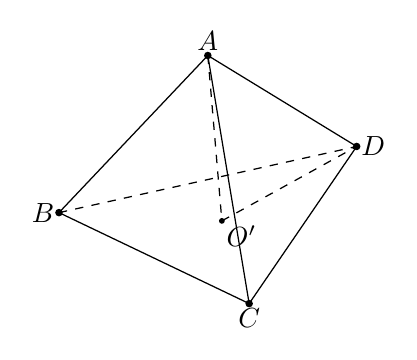
\begin{tikzpicture}[scale=1.05, line width=0.45pt,
  every node/.style={inner sep=1.5pt}]
  \coordinate (A) at (0,1.6);
  \coordinate (B) at (-1.8,-0.3);
  \coordinate (C) at (0.5,-1.4);
  \coordinate (D) at (1.8,0.5);
  \coordinate (Op) at (0.17,-0.4);
  \draw (A) -- (B);
  \draw (A) -- (C);
  \draw (A) -- (D);
  \draw (B) -- (C);
  \draw (C) -- (D);
  \draw[dashed] (B) -- (D);
  \draw[dashed] (A) -- (Op);
  \draw[dashed] (Op) -- (D);
  \fill (A) circle (1.3pt);
  \fill (B) circle (1.3pt);
  \fill (C) circle (1.3pt);
  \fill (D) circle (1.3pt);
  \fill (Op) circle (1pt);
  \node[anchor=south] at (A) {$A$};
  \node[anchor=east] at (B) {$B$};
  \node[anchor=north] at (C) {$C$};
  \node[anchor=west] at (D) {$D$};
  \node[anchor=north west] at (Op) {$O'$};
\end{tikzpicture}
